\chapter{Versatile Interface Adapter}

The \jr\ includes a Western Design Center WDC65C22 versatile interface adapter or VIA. The VIA provides several useful features for I/O and timing:

\begin{itemize}
    \item Two independent I/O ports of eight parallel bits (PA, and PB).

    \item Four handshake control lines (CA1, CA2, CB1, and CB2)

    \item Programmable serial register for serial I/O operations

    \item Two independent timer counters
\end{itemize}

On the \jr, the VIA is connected to header which is compatible with the keyboard header on the Commodore VIC-20 and C-64. This means that a Commodore compatible keyboard could be connected to the \jr\ and used for keyboard input with appropriate programming. The VIA also provides access to the two Atari-style joystick ports. The pins could also be used for general purpose I/O, although the voltage levels are for 3 volt logic instead of the 5 volt logic used in older 8-bit machines.

A complete description of the VIA would be rather long, so this guide will merely list out the register addresses and provide a quick break-down on the register functions. For a complete description, please see the data sheet from Western Design Center.

\begin{table}[h]
    \begin{center}
        \begin{tabular}{|c|c|c|c|c|c|c|c|c|c|c|} \hline
            Address & R/W & Name & 7 & 6 & 5 & 4 & 3 & 2 & 1 & 0 \\\hline\hline
            \verb+0xDC00+ & R/W & IORB & PB7 & PB6 & PB5 & PB4 & PB3 & PB2 & PB1 & PB0 \\ \hline
            \verb+0xDC01+ & R/W & IORA & PA7 & PA6 & PA5 & PA4 & PA3 & PA2 & PA1 & PA0 \\ \hline
            \verb+0xDC02+ & R/W & DDRB & DDRB7 & DDRB6 & DDRB5 & DDRB4 & DDRB3 & DDRB2 & DDRB1 & DDRB0 \\ \hline
            \verb+0xDC03+ & R/W & DDRA & DDRA7 & DDRA6 & DDRA5 & DDRA4 & DDRA3 & DDRA2 & DDRA1 & DDRA0 \\ \hline
            \verb+0xDC04+ & R/W & T1C\_L & T1C7 & T1C6 & T1C5 & T1C4 & T1C3 & T1C2 & T1C1 & T1C0 \\ \hline
            \verb+0xDC05+ & R/W & T1C\_H & T1C15 & T1C14 & T1C13 & T1C12 & T1C11 & T1C10 & T1C9 & T1C8 \\ \hline
            \verb+0xDC06+ & R/W & T1L\_L & T1L7 & T1L6 & T1L5 & T1L4 & T1L3 & T1L2 & T1L1 & T1L0 \\ \hline
            \verb+0xDC07+ & R/W & T1L\_H & T1L15 & T1L14 & T1L13 & T1L12 & T1L11 & T1L10 & T1L9 & T1L8 \\ \hline
            \verb+0xDC08+ & R/W & T2C\_L & T2C7 & T2C6 & T2C5 & T2C4 & T2C3 & T2C2 & T2C1 & T2C0 \\ \hline
            \verb+0xDC09+ & R/W & T2C\_H & T2C15 & T2C14 & T2C13 & T2C12 & T2C11 & T2C10 & T2C9 & T2C8\\ \hline
            \verb+0xDC0A+ & R/W & SR & SR7 & SR6 & SR5 & SR4 & SR3 & SR2 & SR1 & SR0 \\ \hline
            \verb+0xDC0B+ & R/W & ACR & \multicolumn{2}{|c|}{T1\_CTRL} & T2\_CTRL & \multicolumn{3}{|c|}{SR\_CTRL} & PBL\_EN & PAL\_EN \\ \hline
            \verb+0xDC0C+ & R/W & PCR & \multicolumn{3}{|c|}{CB2\_CTRL} & CB1\_CTRL & \multicolumn{3}{|c|}{CA2\_CTRL} & CA1\_CTRL \\ \hline
            \verb+0xDC0D+ & R/W & IFR & IRQF & T1F & T2F & CB1F & CB2F & SRF & CA1F & CA2F \\ \hline
            \verb+0xDC0E+ & R/W & IER & SET & T1E & T2E & CB1E & CB2E & SRE & CA1E & CA2E \\ \hline
            \verb+0xDC0F+ & R/W & IOPA2 & PA7 & PA6 & PA5 & PA4 & PA3 & PA2 & PA1 & PA0 \\ \hline
        \end{tabular}
    \end{center}
    \caption{VIA Registers}
    \label{tab:via_reg}
\end{table}

\begin{description}
    \item[IORA] Input/Output Register for Port A. The eight bits correspond to the eight pins on port A.

    \item[DDRA] Data Direction Register for Port A. Each bit configures the corresponding pin to be input (0) or output (1).

    \item[IORB] Input/Output Register for Port B. The eight bits correspond to the eight pins on port B.

    \item[DDRB] Data Direction Register for Port B. Each bit configures the corresponding pin to be input (0) or output (1).

    \item[T1C] Timer 1 counter value

    \item[T1L] Timer 1 latch

    \item[T2C] Timer 2 counter value

    \item[SR] is the shift register. Serial input may be read here, or data may be written here to be shifted out.

    \item[ACR] Auxiliary Control Register. Contains fields to control the function of timer 1, timer 2, the shift register, and how Port A and Port B latch data.

    \item[PCR] Peripheral Control Register. Contains fields to control how the CA1, CA2, CB1, and CB2 handshake pins are used.

    \item[IFR] Interrupt Flag Register. Contains flags indicating which condition triggered an interrupt request. Possible conditions are timer 1, timer 2, CB1, CB2, CA1, CA2, and shift register complete.

    \item[IER] Interrupt Enable Register. Contains flags to enable or disable interrupts based on the different possible conditions.

    \item[IOPA2] Same as IOPA except that the built-in handshaking capability is not used.

\end{description}

\section{Joystick Support}

The \jr\ has two IDC headers that can be connected to a DB-9 socket to allow Atari style joysticks to be used (see figure:~\ref{fig:joystick_ports} for the pinouts). Joystick header 0 is wired to the pins of Port B, and joystick header 1 is connected to Port A. The various joystick switches are connected to the ports in same manner as on the C-64, with the exception that more buttons are supported (see table:~\ref{tab:via_joystick}).

\begin{figure}[h]
    \begin{center}
        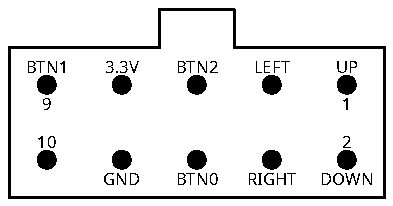
\includegraphics{images/f256jr_joystick_pinout.pdf}
    \end{center}
    \caption{Joystick Port Pinouts}
    \label{fig:joystick_ports}
\end{figure}

In order to use the joysticks, the DDR bits for the ports must be set to 0 for input. Then the input/output register for the port may be read. If a button or switch is closed on the joystick, the corresponding bit in the I/O register will be clear (0). If the button is not pressed, the bit will be set (1).

As a reminder: be aware that the WDC65C22 on the \jr\ is being used with a 3 volt supply. This means that any device plugged into the joystick ports should be 3 volt tolerant and should not raise any pin above 3 volts. Otherwise damage could occur.

\begin{table}[h]
    \begin{center}
        \begin{tabular}{|c|c|c|c|c|c|c|c|} \hline
            7 & 6 & 5 & 4 & 3 & 2 & 1 & 0 \\\hline
            --- & BUTTON2 & BUTTON1 & BUTTON0 & RIGHT & LEFT & DOWN & UP \\ \hline
        \end{tabular}
    \end{center}
    \caption{Joystick Flags}
    \label{tab:via_joystick}
\end{table}

\example{Displaying Joystick 1}
In this example, we will poll joystick 1 and print out the state of all the buttons by printing the byte we read from the joystick port as a simple binary number. The example will try to be a little bit smart by only printing the value when the value has changed. NOTE: this example expects OpenKernal to be installed, and will call two of its routines for initializing the screen and printing a character.

First, we initialize the screen, the variable we use to track the old value of the joystick port, and the VIA (setting port A to be an input port):
\begin{verbatim}
ok_cint = $FF81                         ; OpenKernal routine to initialize the screen
ok_cout = $FFD2                         ; OpenKernal routine to print a character in A

; Variables

* = $0080

value:      .byte ?                     ; Variable to store the previous value of the joystick
prv:        .byte ?                     ; Copy of value for printing

* = $e000

start:      jsr ok_cint                 ; Set up the screen

            lda #$FF                    ; Set the previous value to $FF
            sta value

            stz MMU_IO_CTRL             ; Switch to I/O Page 0

            lda #$00                    ; Set VIA Port A to input
            sta VIA_DDRA
\end{verbatim}

Next, we print the OpenKernal code to clear the screen, and we print out the byte in \verb+value+ as a binary number.

\begin{verbatim}
loop1:      lda #147                    ; Print the CBM clear screen code
            jsr ok_cout

            lda value                   ; Copy the value to prv
            sta prv

            ldx #8                      ; Loop for all eight bits
loop2:      asl prv                     ; Shift MSB into the carry
            bcc is0                     ; If it's 0, print '0'

            lda #'1'                    ; Otherwise, print '1'
            jsr ok_cout
            bra repeat                  ; And go to the next bit

is0:        lda #'0'                    ; Print '0'
            jsr ok_cout

repeat:     dex                         ; Count down
            bne loop2                   ; Repeat until we've done all 8 bits
\end{verbatim}

Next, we read the value of port A. If it is different from \verb+value+, we save it to \verb+value+ and go back to print the byte we read. Otherwise, we keep waiting and polling the joystick port.

\begin{verbatim}
            stz MMU_IO_CTRL             ; Switch to I/O Page 0

wait:       lda VIA_IORA                ; Get the status of port A
            cmp value                   ; Is it different from before?
            beq wait                    ; Yes: keep waiting

            sta value                   ; Save this value as the previous one
            bra loop1                   ; And go to print it
\end{verbatim}
